
\chapter{Содержание}

\textit{Цель работы}: построение гистограммы и эмпирической функции распределения.
\begin{itemize}
	\item Для выборки объема n из генеральной совокупности X реализовать в виде программы на ЭВМ:
	\begin{enumerate}
		\item вычисление максимального значения $M_{max}$ и минимального значения $M_{min}$;
		\item размаха $R$ выборки;
		\item вычисление оценок $\hat{\mu}$ и $S^2$ математического ожидания MX и дисперсии DX;
		\item группировку значений выборки в $m = [\log_2n] + 2$ интервала;
		\item построение на одной координатной плоскости гистограммы и графика функции плотности распределения вероятностей нормальной случайной величины с математическим ожиданием $\hat{\mu}$ и дисперсией $S^2$;
		\item построение на другой координатной плоскости графика эмпирической функции распределения и функции распределения нормальной случайной величины с математическим ожиданием $\hat{\mu}$ и дисперсией $S^2$.
	\end{enumerate}
	\item Провести вычисления и построить графики для выборки из индивидуального варианта.
\end{itemize}


\chapter{Теория}

Пусть $\vec{x} = (x_1, \dots, x_n)$ --- реализация случайной
выборки из генеральной совокупности X. n --- объем выборки.

\begin{enumerate}[wide=0pt]
	\item Максимальное значение выборки: $M_{max} = \max{(x_1, x_2, \dots, x_n)},$

	\item Минимальное значение выборки: $M_{min} = \min{(x_1, x_2, \dots, x_n)},$

	\item Размах выборки: $R = M_{max} - M_{min},$

	\item Оценка математического ожидания: $\hat{\mu}(\vec{X}) = \cfrac{1}{n}\sum_{i = 1}^{n}x_i,$

	\item Оценка дисперсии: $S^2(\vec{X}) = \cfrac{1}{n}\sum_{i = 1}^{n}(x_i - \bar{x})^2.$
\end{enumerate}



	Расположим значиения $x_1, x_2, \dots, x_n$ в порядке неубывания.
\begin{equation}
	x_{(1)}, x_{(2)}, \dots, x_{(n)}
\end{equation}

	$x_{(i)}$ --- это элемент вариационного ряда.

	\textit{Интервальный статистический ряд} --- это ряд $J = [x_{(i)}, x_{(n)}]$, 
	который разбивают на $m$ промежутков, 
	ширина которых определяется согласно \ref{delta}:

	\begin{equation}\label{delta}
	\Delta = \cfrac{\left|J\right|}{m} = \cfrac{R}{m},
\end{equation}
\begin{equation}
	\begin{array}{ll}
		J_i = \left[x_{(1)} + \left(i - 1\right)\Delta; \; x_{(i)} + i\Delta\right), \; i = \overline{1,\: m - 1},\\
		J_m = \left[ x_{(1)} + \left(m - 1\Delta\right), \; x_{(n)}\right).
	\end{array}
\end{equation}

\textit{Эмпирической плотностью} распределения соответствующей выборке $\vec{x}$ называется функция \ref{cdf}:
\begin{equation}\label{cdf}
	f_n(x) = 
	\begin{cases}
		\cfrac{n_i}{n \cdot \Delta} & ,x \in J_i, \\
		0 & ,\text{иначе.}
	\end{cases}
\end{equation}

где $n_i$ --- количество значений выборки в J, интервале интервального ряда.
$\Delta$ --- длина интервала.

Гистограмма --- график эмпрической функции плотности распределения. 

$n(t, \vec{x})$ -- число компонент вектора $\vec{x}$, которые меньше чем $t$. \textit{Эмпирической функцией распределения}, построенной по выборке $\vec{x}$ называется функция $F_n: \mathbb{R} \rightarrow \mathbb{R}$, определенная правилом \ref{pdf}.

\begin{equation}\label{pdf}
	F_n(t) = \cfrac{n(t, \vec{x})}{n}
\end{equation}

\chapter{Результаты}

\begin{figure}[ht!]
	\begin{center}
		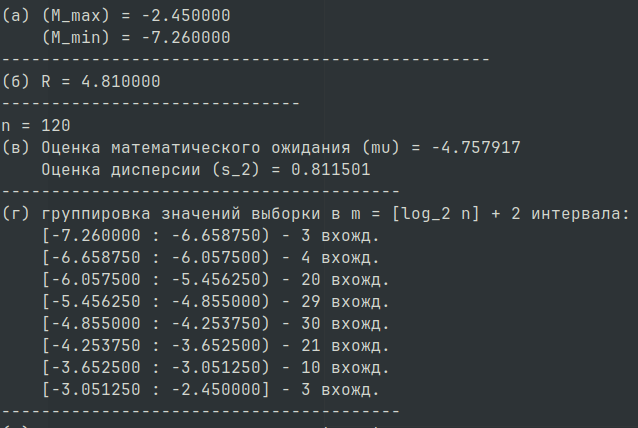
\includegraphics[scale=0.5]{assets/launch.png}
		\caption{Результат работы программы}
	\end{center}
\end{figure}

\begin{figure}[ht!]
	\begin{center}
		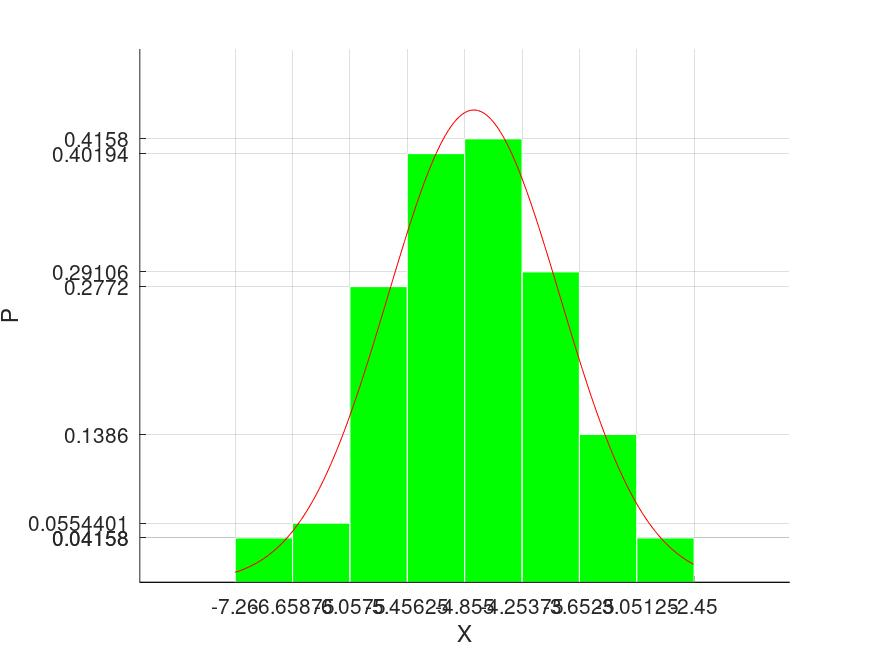
\includegraphics[scale=0.4]{assets/hist.jpg}
		\caption{Гистограмма и график функции плотности распределения вероятностей нормальной случайной величины}
	\end{center}
\end{figure}

\begin{figure}[ht!]
	\begin{center}
		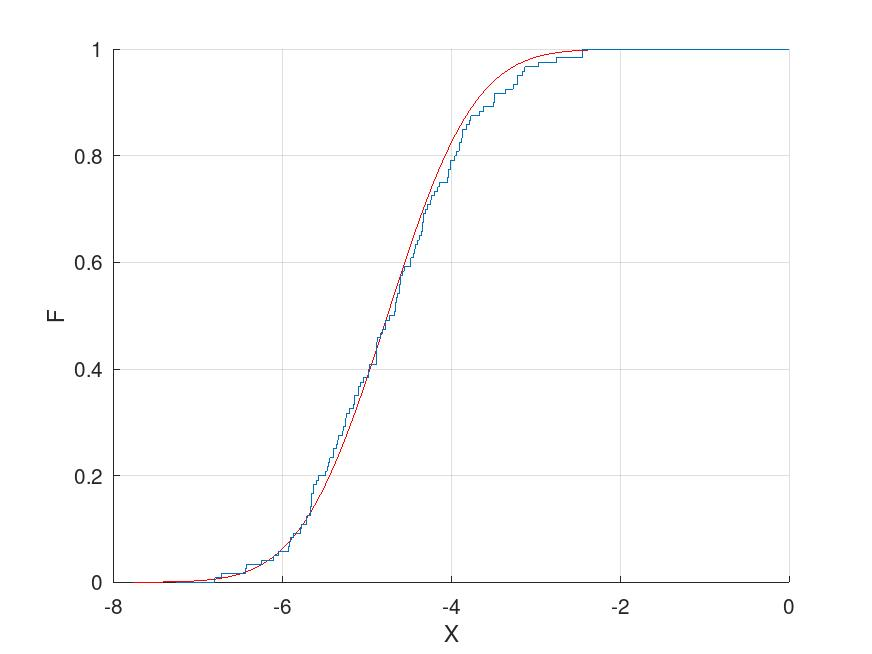
\includegraphics[scale=0.4]{assets/cdf.jpg}
		\caption{График эмпирической функции распределения и функции распределения нормальной случайной величины}
	\end{center}
\end{figure}